\subsubsection{Reranker}
\label{subsubsec:reranker}

After all of the previous steps, we obtained a working system that achieved satisfactory results at a good speed, so we tried to improve it by introducing a second stage, called \textit{passage re-ranking}, in which each of the documents returned by the first retrieval model would be scored and re-ranked by a more computationally-intensive method involving Machine Learning. \\
\begin{figure}[tbp]
  \centering
  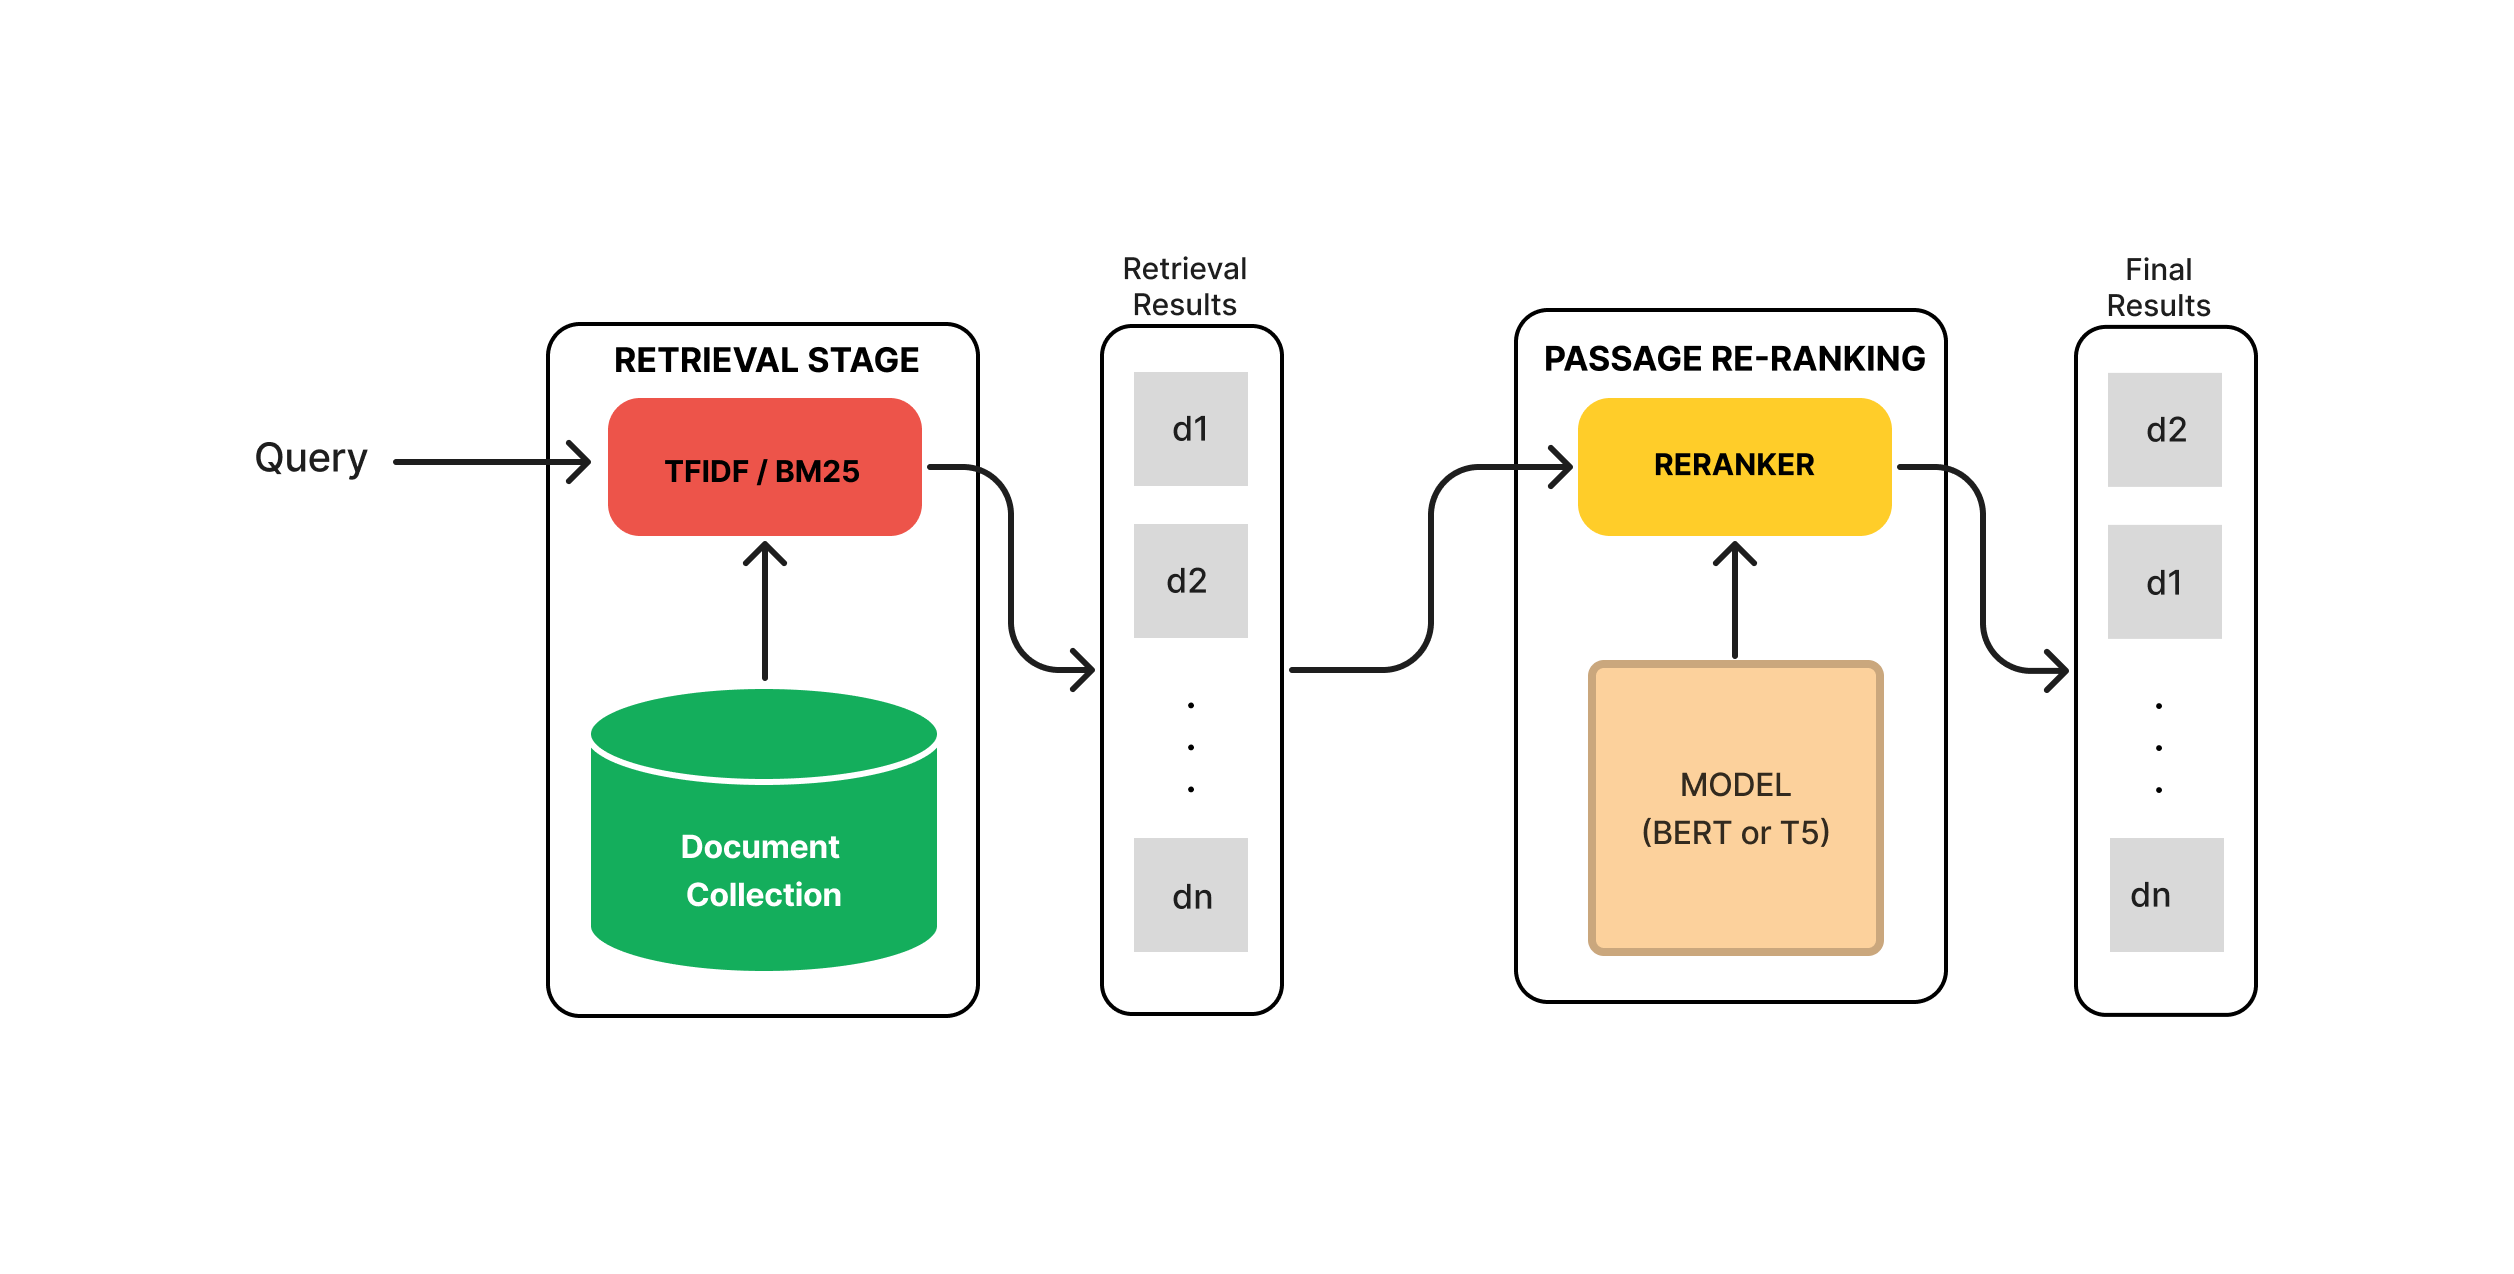
\includegraphics[width=0.8\linewidth]{figure/rerank_framework.png}
  \caption{Retrieve-than-rerank framework}
  \label{fig:rerank}
\end{figure}
We achieved this by leveraging a library called PyGaggle\footnote{https://github.com/castorini/pygaggle}, which provides some deep neural architectures for text ranking and question answering, and two transformer-based models, T5 and BERT, with different checkpoints and even our own trained checkpoint using code from another library \cite{gao2021lce}.

In our system, we can choose how many documents are to be reranked from the top for two reasons: the first is raw computing performance, reranking all 1000 retrieved documents takes a long time and we don't have machines powerful enough to handle it; the second is that we saw that reranking more than 50 documents lowers our measures, even below the baseline measure without reranking.\\
Our first approach to reranking was to consider only the scores returned by the models to rerank the documents but we then switched to an approach where we consider also the BM25 score as follows. Let $Score_{BM25}(i)$ the score given by BM25 for the document at rank $i$ and $Score_{rr}(i)$ the score given by the reranker for the document at rank $i$, and let $n$ be the total number of reranked documents, we define: 
\begin{equation}
nScore_{rr}(i) = \bigg(Score_{rr}(i)+\min_{j\in [1,n]}Score(j)\bigg)\cdot \frac{Score_{BM25}(1)}{Score_{rr}(1)}
\end{equation}
as the normalized score for the reranked documents, since the models returned a score in the range $[-10,+10]$, which was not suitable for our case.\\
In our first approach, we simply passed the score to Lucene's \texttt{ScoreDoc} object and we were done. But in this way, we would lose information about the ranking given by BM25, which is still relevant, so we defined a new score: 
\begin{equation}
finalScore(i) = mntr + (1-\alpha)\cdot Score_{BM25}(i)+\alpha\cdot nScore_{rr}(i)
\end{equation}
where $mntr$ is the maximum score from docs which are not reranked, in this way, we preserve the order of this docs. With this approach, we can give a weight to the reranker to find the balance and we do not lose the information given to us by the first stage. Note that $\alpha=1$ corresponds to considering only scores from the reranker.

\noindent \textbf{Pretrained Models}

We tried two transformer-based models, T5 and BERT since they are supported by PyGaggle. First, we tried T5 \cite{RaffelShazeerRobertsLeeNarangMatenaZhouLiLiuT5}, but with BERT \cite{devlin2019bert} we got better results. Starting from the same base model, t5-base\footnote{https://huggingface.co/t5-base} for T5 bert-base-uncased\footnote{https://huggingface.co/bert-base-uncased} for BERT, we tried different checkpoints\footnote{saving the model's parameters and optimizer state during the training process} fine-tuned specifically for reranking tasks and we even tried to train our checkpoint. The pre-trained checkpoints that we used are: 
\begin{itemize}
\item \textit{monot5-base-msmarco-10k}\footnote{https://huggingface.co/castorini/
monot5-base-msmarco-10k}
\item \textit{bert-base-mdoc-bm25}\footnote{https://huggingface.co/Luyu/
bert-base-mdoc-bm25}
\end{itemize}
The results for the T5 model are reported in Table~\ref{tab:t5-msmarco} and the results for the BERT model are reported in Table~\ref{tab:bert-mdoc}.
\begin{table}[tbp]
\caption{\label{tab:t5-msmarco} monot5-base-msmarco-10k model with different number of documents to rerank}
\begin{tabular}{|l|l|l|}
\toprule
             & \textbf{nDCG} & \textbf{MAP} \\ 
\midrule
\textbf{0}   & 0.4075        & 0.2411       \\ 
\textbf{10}  & \textbf{0.414}         & \textbf{0.2502}       \\ 
\textbf{20}  & 0.4119        & 0.2477       \\ 
\textbf{50}  & 0.4083        & 0.242        \\ 
\textbf{100} & 0.405         & 0.2376       \\ 
\textbf{250} & 0.3987        & 0.2301\\
\bottomrule
\end{tabular}
\end{table}

\begin{table}[tbp]
\caption{\label{tab:bert-mdoc}bert-base-mdoc-bm25 model with different number of documents to rerank}
\begin{tabular}{|l|l|l|}
\toprule
             & \textbf{nDCG} & \textbf{MAP} \\ 
\midrule
\textbf{0}   & 0.4075        & 0.2411       \\ 
\textbf{10}  & 0.4207         & 0.2608       \\ 
\textbf{20}  & \textbf{0.4222}        & \textbf{0.2617}       \\ 
\textbf{50}  & 0.4212        & 0.2598        \\ 
\textbf{100} & 0.4184         & 0.2563       \\ 
\textbf{250} & 0.4104        & 0.2478      \\
\bottomrule
\end{tabular}
\end{table}
The BERT pretrained checkpoint with 20 reranked documents improved \ac{nDCG} by $3.56\%$ and \ac{MAP} by $8.5\%$.

\noindent \textbf{Training our own checkpoint}\\
At this point, BERT gave us good results so we took it a step further and we tried to find ways to finetune it to our data. The training process is pretty straightforward: 
\begin{itemize}
\item \textbf{Data pre-processing}. Transformers expect batches of tensors as input, so we need to preprocess our data to the expected format. For processing textual data the tokenizer tool is used, which splits text into tokens; in our case, we exploit the pre-trained BERT tokenizer which returns tokens that are not necessarily words, but rather subwords: frequently used words are (or should) not split into smaller subwords, but rare words should be decomposed into meaningful subwords \cite{HfTokenizer}. Further, the tokenizer adds, at the beginning and at the end, two special tokens, respectively \texttt{[CLS]} and \texttt{[SEP]}. The tokenizer returns a dictionary with three items: 
	\begin{itemize}
		\item \texttt{input\_ids}, indices corresponding to each token in the sentence
		\item \texttt{attention\_mask}, indicates whether a token should be attended to or not
		\item \texttt{token\_type\_ids}, identifies which sequence a token belongs to when there is more than one sequence
	\end{itemize}
An important note is that BERT accepts input sequences of up to 512 tokens, so the tokenizer truncates longer documents. 
\item \textbf{Training}. The easiest way to train is to use the Trainer\footnote{https://huggingface.co/docs/transformers/main\_classes/
trainer} API from PyTorch.
\end{itemize} 
To ease development, we used a package for training deep language model rerankers \cite{gao2021lce} and adapted the example code to our collection.

The \texttt{convert\_to\_training.py} takes care of converting data to the training file, given the ranking file, the qrels, the query collection and the docs collection. Then it is sufficient to use the \texttt{trainer.py} code to get the trained model. Unfortunately, we don't have access to sufficiently powerful machines so we were forced to train on a Google Colab notebook. This came with a major drawback: the maximum runtime is 12 hours, so we couldn't train on more than 1 epoch since a 2 epoch model was estimated to take 15 hours to train. This obviously tanked our model performances, and, as we can see in Table~\ref{tab:own-model}.

\begin{table}[tbp]
\caption{\label{tab:own-model}Our trained model with different number of documents to rerank}
\begin{tabular}{|l|l|l|}
\toprule
             & \textbf{nDCG} & \textbf{MAP} \\
\midrule
\textbf{0}   & 0.4075        & 0.2411       \\ 
\textbf{10}  & 0.3910         & 0.2253       \\ 
\textbf{20}  & 0.3741       & 0.1975       \\ 
\textbf{50}  & 0.3405        & 0.1580        \\ 
\bottomrule
\end{tabular}
\end{table}

\noindent The Colab notebook with all the hyperparameters can be found at \url{https://colab.research.google.com/drive/1oFeYSkR31A-MUibwWrfNcKLUyPxEYbOq?usp=sharing}.
The trained model can be found at \url{https://huggingface.co/enricobolzonello/clef_longeval}.

\noindent \textbf{Integrating with Lucene}\\
One problem that emerged while working with the reranker was integrating it with Lucene since the reranker is written in Python and our main program is in Java. To solve the issue we came up with three approaches: 
\begin{enumerate}
\item passing intermediate text files, with documents, query to the reranker and returning the ranking to Java. This solution was used for initial testing but was deemed too inefficient and prone to errors
\item using Python as the system's entry point and using the PyJNIus\footnote{https://github.com/kivy/pyjnius} library to access Java classes. The same approach was used by Birch \cite{Birch}, but we should have changed the classes too much to integrate tightly the reranker and more importantly we didn't want to change the entry point of our system 
\item our final solution was to call in some way Python from Java
\end{enumerate}
The library we used to achieve this is JEP\footnote{https://github.com/ninia/jep}, which uses \ac{JNI} and the CPython API to start up the Python interpreter inside the \ac{JVM}. Thanks to the Python interpreter, we can call, at each query, the reranker which returns a list of generic \texttt{Object}s that is converted to a list of \texttt{Float}.